\Chapter{Chapter 2}{Creating graphs from data}{Chapter 2: Creating graphs from data}

\fancyhead[R]{\fontsize{12}{14}\selectfont\textit{Chapter 2: Creating graphs from data}}

\chaptertitle{Chapter 2: Creating graphs from data}

\learningobjectives{
    \item Creating a histogram by hand and in R
    \item Creating and modifying a scatter plot in R
    \item Creating and modifying a line plot in R
    \item Creating a box plot in R
}

% To add an assignment to the chapter, create a file in the folder "Assignments" and insert the link below

%%%%%%%%%%%%%%%%%%%%%%%%%%%%%%%%%%%%%%%%%%%%%%%%%%%%%%%%%%%%%%%%%%%%%%%%%%%
% Assignment 2.1: Creating a histogram by hand
%%%%%%%%%%%%%%%%%%%%%%%%%%%%%%%%%%%%%%%%%%%%%%%%%%%%%%%%%%%%%%%%%%%%%%%%%%%

\handassignment{Assignment 2.1: Creating a histogram by hand}

Suppose that you have the following set of numbers: \\

\begin{center}
\hspace{0.3cm}1.5\hspace{0.3cm}5.5\hspace{0.3cm}1.7\hspace{0.3cm}7.2\hspace{0.3cm}1.2\hspace{0.3cm}7.9\hspace{0.3cm}1.4\hspace{0.3cm}3.6\hspace{0.3cm}3.1\hspace{0.3cm}3.8\hspace{0.3cm}5.9\hspace{0.3cm}3.6\hspace{0.3cm}5.1\hspace{0.3cm}3.2\hspace{0.3cm}7.1
\end{center}

\question{
    2.1 a
}{
    For each of the ranges given below, find out their \concept{frequency} in the data above.
}

\emptyanswerbox{
    2.1a
}{
    \begin{center}
    \begin{tabular}{|c|c|c|c|}
    \hline
    0 to 2 & 2 to 4 & 4 to 6 & 6 to 8 \tstrut\bstrut\\
    \hline
    & & & \\
    Frequency:\hspace*{2pt}\rule{0.8cm}{0.4pt}  & Frequency:\hspace*{2pt}\rule{0.8cm}{0.4pt} & Frequency:\hspace*{2pt}\rule{0.8cm}{0.4pt} & Frequency:\hspace*{2pt}\rule{0.8cm}{0.4pt} \bstrut\\
    \hline
    \end{tabular}
    \end{center}
}

\question{
    2.1 b
}{
    Draw the histogram for these data by hand. The name of the \textit{x-axis} should represent the range of values, and the name of the \textit{y-axis} should represent the \concept{frequency} of the values that fall in the ranges of assignment 2.1a.
}

\emptyanswerbox{
    2.1 b
}{
    \vspace*{-0.5cm}
    \begin{center}
    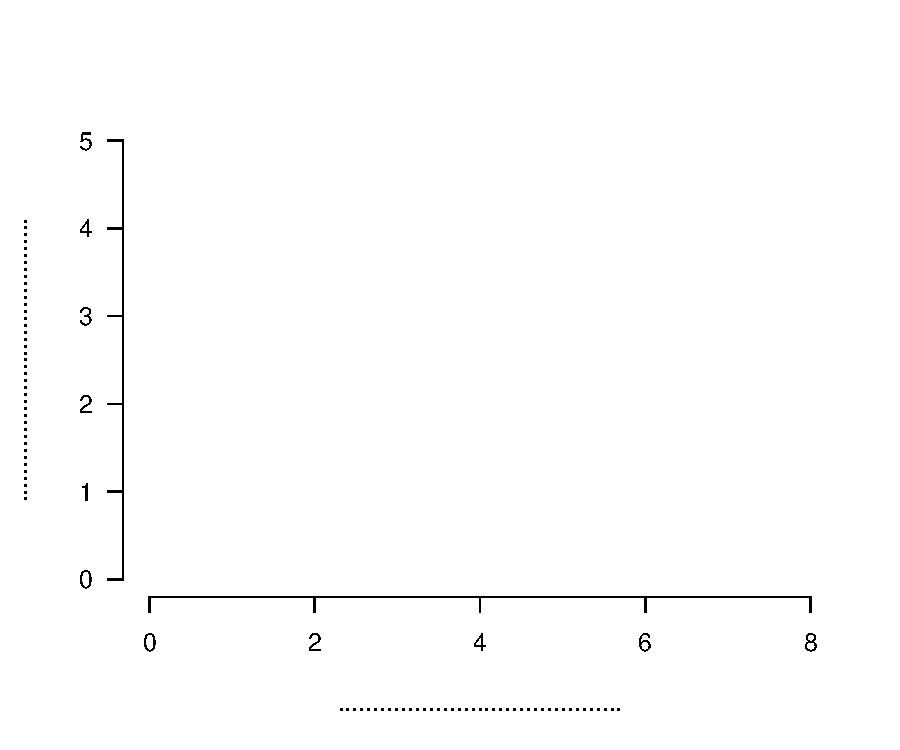
\includegraphics[height = 7cm]{Files/Images/emptyHistogram.pdf}
    \end{center}
}

\clearpage % Page break
%%%%%%%%%%%%%%%%%%%%%%%%%%%%%%%%%%%%%%%%%%%%%%%%%%%%%%%%%%%%%%%%%%%%%%%%%%%
% Assignment 2.2: Creating and modifying a histogram in R
%%%%%%%%%%%%%%%%%%%%%%%%%%%%%%%%%%%%%%%%%%%%%%%%%%%%%%%%%%%%%%%%%%%%%%%%%%%

\rassignment{Assignment 2.2: Creating and modifying a histogram in R}

\question{
    2.2 a
}{
    Take the numbers from assignment 2.1a and use the \rcode{c()} function to enter these numbers in a vector called \rcode{dataset4}. Next, run the following code in \texttt{R} and explain what you see.
}

\codeblock{hist(dataset4)}

\twolineanswerbox{2.2a}

\question{
    2.2 b
}{
    The graph resulting from the command in 2.2a is not the same as the histogram that you drew in assignment 2.1b. What is the difference between the graph from 2.2a and your graph from 2.1b? 
}

\twolineanswerbox{2.2b}

\question{
    2.2 c
}{
    Try to replicate your \underline{exact} histogram from 2.1b in \texttt{R}. This requires that you specify the \rcode{breaks} argument after a comma in the \rcode{hist()} function. 
}

\hint{Hint 2.1: You can find more information on the \rcode{hist()} function by running \rcode{?hist}.}

\rcodeanswertiny{2.2c}

\question{
    2.2 d
}{
    Give your histogram a different color by adding and changing the \rcode{col} argument after the comma. Improve your histogram further by changing the \textit{x-axis} name, the main title, and the rotation of the \textit{y-axis} labels by adding more arguments.
}

\hint{Hint 2.2: Check Part II of the R help for additional arguments to the \rcode{hist()} function.}

\rcodeanswersmall{2.2d}

\question{
    2.2 e
}{
    Calculate the \concept{mean} and \concept{median} of the values of \rcode{dataset4}. Is the distribution of \rcode{dataset4} \concept{negatively skewed} or \concept{positively skewed}? Explain your answer using the relation between the \concept{mean} and the \concept{median}.
}

\emptyanswerbox{
    2.2e
}{
    These data sets are \textbf{positively} / \textbf{negatively} / \textbf{not} skewed.
    \answerskip
    Explanation:
    \answerskip
    \rule{\textwidth}{0.4pt}
    \answerbreak
    \rule{\textwidth}{0.4pt}
    \answerbreak
    \rule{\textwidth}{0.4pt}
}

\clearpage % Page break
%%%%%%%%%%%%%%%%%%%%%%%%%%%%%%%%%%%%%%%%%%%%%%%%%%%%%%%%%%%%%%%%%%%%%%%%%%%
% Assignment 2.3: Creating and modifying a scatter plot in R
%%%%%%%%%%%%%%%%%%%%%%%%%%%%%%%%%%%%%%%%%%%%%%%%%%%%%%%%%%%%%%%%%%%%%%%%%%%

\rassignment{Assignment 2.3: Creating and modifying a scatter plot in R}

In this assignment you are going to work with a data set that is built into \texttt{R}. \\

The \rcode{data()} function gives you access to all the data sets that are built into \texttt{R}, or that are included with downloaded \texttt{R} packages. For example, you can load a data set called \rcode{swiss} into the environment by running the \texttt{R} code below: \\

\codeblock{data(swiss)} 

The data are imported as an object called \rcode{swiss}, which you can now also see in the environment. This particular data set contains some socio-economic indicators for each of 47 French-speaking provinces of Switzerland. In this assignment, you will focus on the column \rcode{Education} (the percentage education beyond primary school) and the column \rcode{Agriculture} (the percentage of males involved in agriculture as an occupation). \\

\question{
    2.3 a
}{
    Extract the values of the two columns using the \rcode{\$} sign and store them in two new variables called \rcode{education} and \rcode{agriculture}.
}

\hint{Hint 2.3: You can check the R environment to see the names of the objects that you have currently stored.}

\rcodeanswertiny{2.3a}

\question{
    2.3 b
}{
    Use the \rcode{plot()} function to create a scatter plot of the two variables. Place the percentage of education beyond primary school on the \textit{x-axis} and the percentage of males involved in agriculture as an occupation on the \textit{y-axis}. Rename your axis labels to match the content of the graph.
}

\rcodeanswerlarge{2.3b}

\clearpage % Page break

\question{
    2.3 c
}{
    Looking at the scatter plot, what can you globally say about the relation between the percentage of education beyond primary school and the percentage of males involved in agriculture as an occupation in the French-speaking provinces of Switzerland? 
}

\twolineanswerbox{2.3c}

\question{
    2.3 d
}{
    Give the points in your scatter plot a different color by changing the \rcode{col} argument after the comma. Improve the graph further by changing the main title, the rotation of the \textit{y-axis} labels, the shape of the points, and removing the outer lines.
}

\rcodeanswerlarge{2.3d}

\clearpage % Page break
%%%%%%%%%%%%%%%%%%%%%%%%%%%%%%%%%%%%%%%%%%%%%%%%%%%%%%%%%%%%%%%%%%%%%%%%%%%
% Assignment 2.4: Creating and modifying a line plot in R
%%%%%%%%%%%%%%%%%%%%%%%%%%%%%%%%%%%%%%%%%%%%%%%%%%%%%%%%%%%%%%%%%%%%%%%%%%%

\rassignment{Assignment 2.4: Creating and modifying a line plot in R}

In this assignment, you are going to create a line plot of the daily closing prices of some major European stock indices: Germany DAX, Switzerland SMI, France CAC, and UK FTSE. \\

You can load this data set by running the code below: \\

\codeblock{data(EuStockMarkets) \\
            stockData <- data.frame(EuStockMarkets)
}

The data is now loaded into the environment as the \rcode{EuStockMarkets} data set and immediately transformed to the \rcode{stockData} data set (this is because of technical reasons as the original data is in a time-series format). In this assignment, you will work with the \rcode{stockData} data set. \\

\question{
    2.4 a
}{
    Create a line plot where the closing price of the DAX stock is displayed over time. Give your plot appropriate \textit{x-axis} and \textit{y-axis} names.
}

\rcodeanswersmall{2.4a}

\question{
    2.4 b
}{
    Find a function to add a separate line for the closing price of the SMI stock in red. You may try to add the other stocks as well using this function, but remember to adjust the \textit{y-axis} accordingly so that all the lines are all displayed decently.
}

\hint{Hint 2.4: Do \underline{not} use the \rcode{plot()} function to add a line to an already existing plot.}

\rcodeanswersmall{2.4 b}

\clearpage % Page break
%%%%%%%%%%%%%%%%%%%%%%%%%%%%%%%%%%%%%%%%%%%%%%%%%%%%%%%%%%%%%%%%%%%%%%%%%%%
% Assignment 2.5: Creating a box plot in R
%%%%%%%%%%%%%%%%%%%%%%%%%%%%%%%%%%%%%%%%%%%%%%%%%%%%%%%%%%%%%%%%%%%%%%%%%%%

\rassignment{Assignment 2.5: Creating a box plot in R}

For this next assignment, let’s return to the \rcode{swiss} data set. More specifically, you will now have to focus on the values that are stored in the separate variable \rcode{agriculture}. \\

\question{
    2.5 a
}{
    Find out the \concept{minimum}, \concept{lower quartile}, \concept{median}, \concept{upper quartile}, and \concept{maximum} of the \rcode{agriculture} variable.
}

\rcodeanswersmall{2.5a}

\emptyanswerbox{
    2.5a
}{
    Minimum: \quad \shortanswerline \quad Upper quartile: \shortanswerline
            \answerskip
            Median: \quad\hspace*{7pt} \shortanswerline \quad Lower quartile: \shortanswerline
            \answerskip
            Maximum: \quad \shortanswerline
}

\question{
    2.5 b
}{
    Create a boxplot of the \rcode{agriculture} variable.
}

\rcodeanswertiny{2.5b}

\question{
    2.5 c
}{
    Run the following code in \texttt{R} and explain the table output. How does the code work?
}

\codeblock{educationLevel <- rep(\textquotesingle2.Medium\textquotesingle, 47)\\
educationLevel[education <= 6] = \textquotesingle1.Low\textquotesingle\\
educationLevel[education >= 12] = \textquotesingle3.High\textquotesingle\\
table(educationLevel)
}

\twolineanswerbox{2.5c}

\clearpage % Page break

\question{
    2.5 d
}{
    Create a box plot using the \texttt{R} code below and explain what you see.
}

\codeblock{boxplot(agriculture {\raise.17ex\hbox{$\scriptstyle\sim$}} educationLevel)}

\twolineanswerbox{2.5d}

\clearpage % Page break

\vspace*{2cm}
\fancyhf[rh]{}
\begin{center}
    \textit{This page is intentionally left blank}
\end{center}

\clearpage % Page break